\section{实验原理}
\subsection{基本光学原理}
\frame{\frametitle{折射率与密度}
光在不同介质中的传播速度是不同的, 与介质的折射率$n$有关.
\[
n = \frac{c}{v} = 1 + \frac{c-v}{v} = 1 + \frac{\Delta\lambda}{\lambda}
\]

对于一定的介质, 其折射率是介质密度的函数, 当n接近为1时, 通常可以将上式近似表达为:
\[
\frac{n-1}{\rho} = K_{GD} {~}\textrm{或}{~} n=1+K_{GD}\rho
\]
上式称为Gladstone-Dale公式, 其中$K_{GD}$为常数, 是气体的一种特性, 称为比折射度. 一般情况下, 气体密度$\rho$与气体折射率$n$的关系可用上述Gladstone-Dale公式表示.
}

\frame{\frametitle{光线传输过程中的三个变量}
\begin{center}
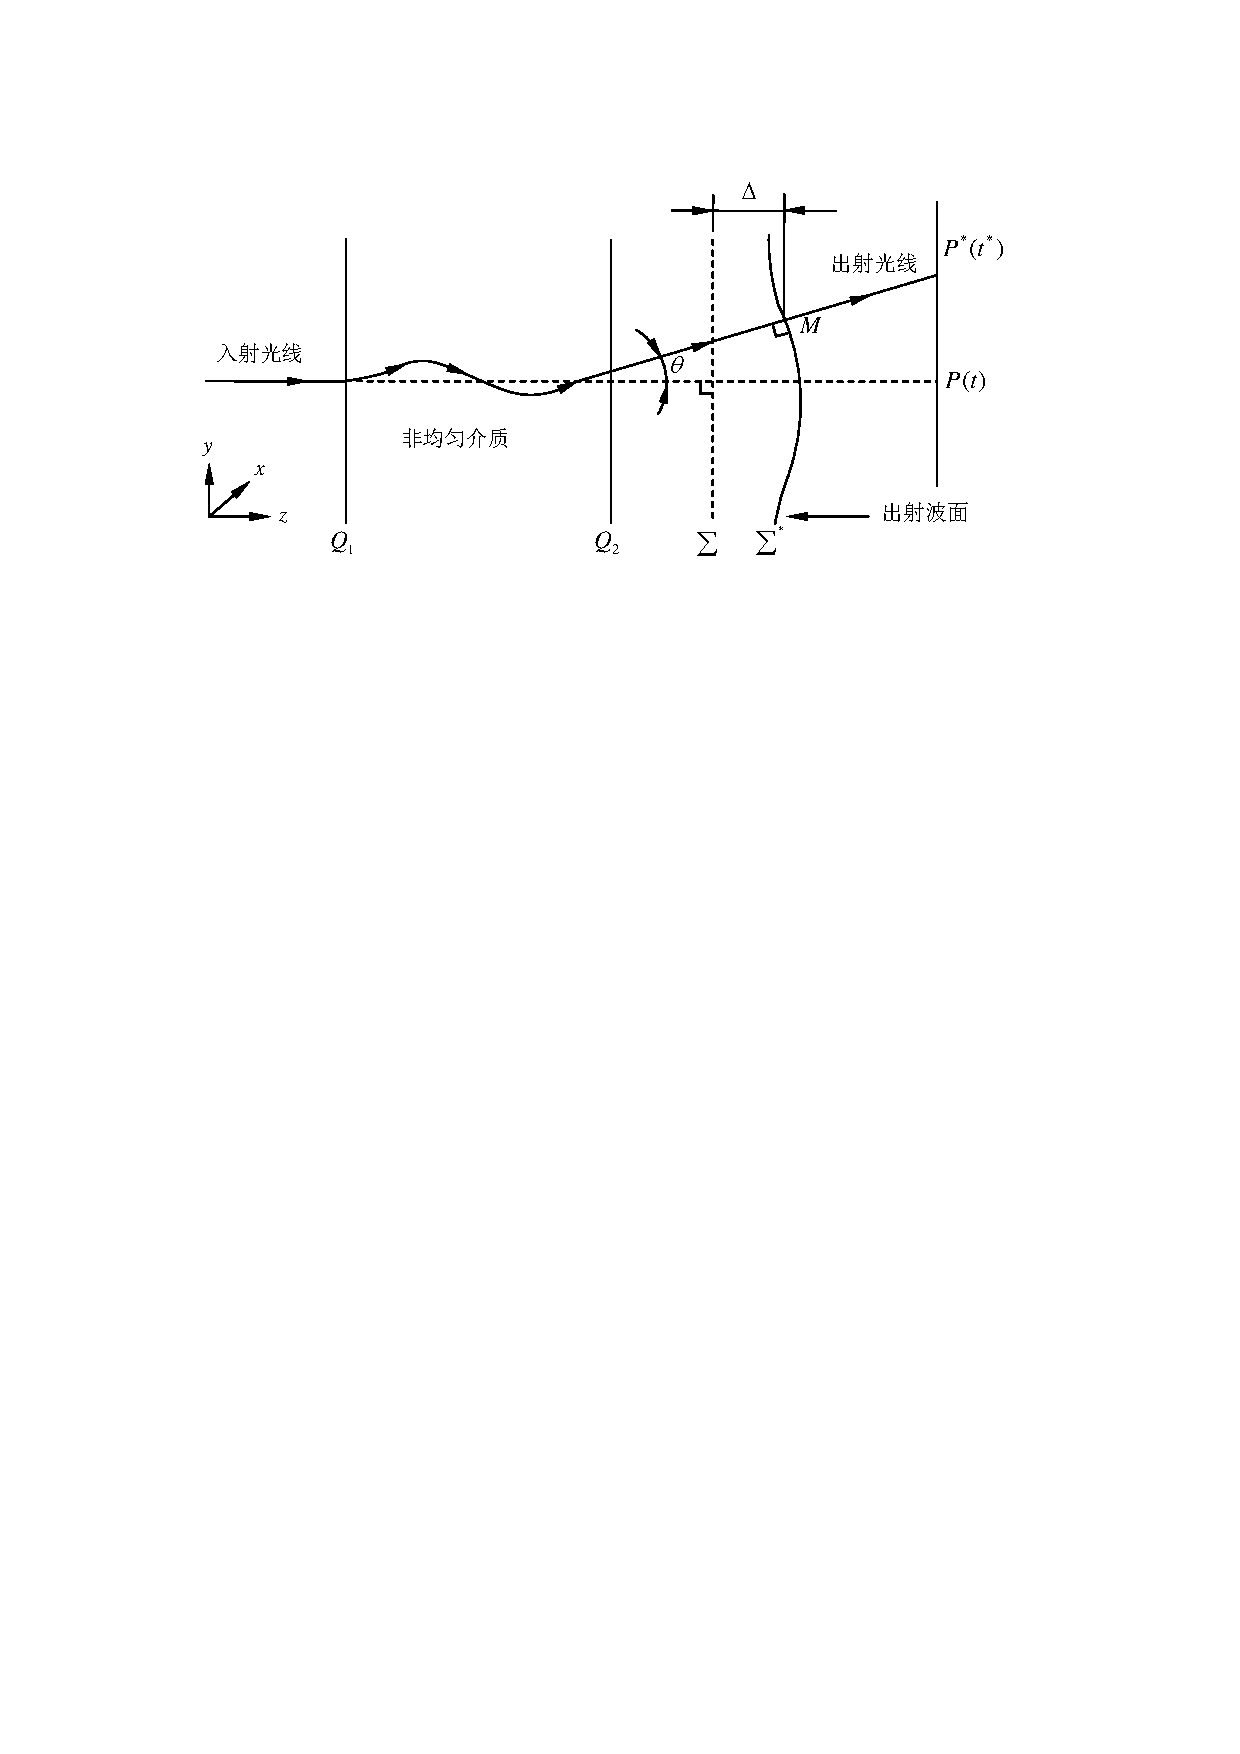
\includegraphics[width=0.9\textwidth]{optics.pdf}\\
\vspace{1em}

\textcolor{blue}{
\begin{tabular}{lll}
接收屏上的光线位移量($P^*P$) &  & $\partial^2\rho/\partial x^2$ \\
扰动与未扰动光线间的角偏移($\theta^*-\theta$) &   & $\partial\rho/\partial x$\\
光线的光程差引起的相位变化($\varphi^*-\varphi$) &  & $d\rho/dt$ \\
\end{tabular}
}
\end{center}
}

\subsection{阴影法}
\frame{\frametitle{阴影法}
\begin{columns}
\begin{column}[c]{0.5\textwidth}
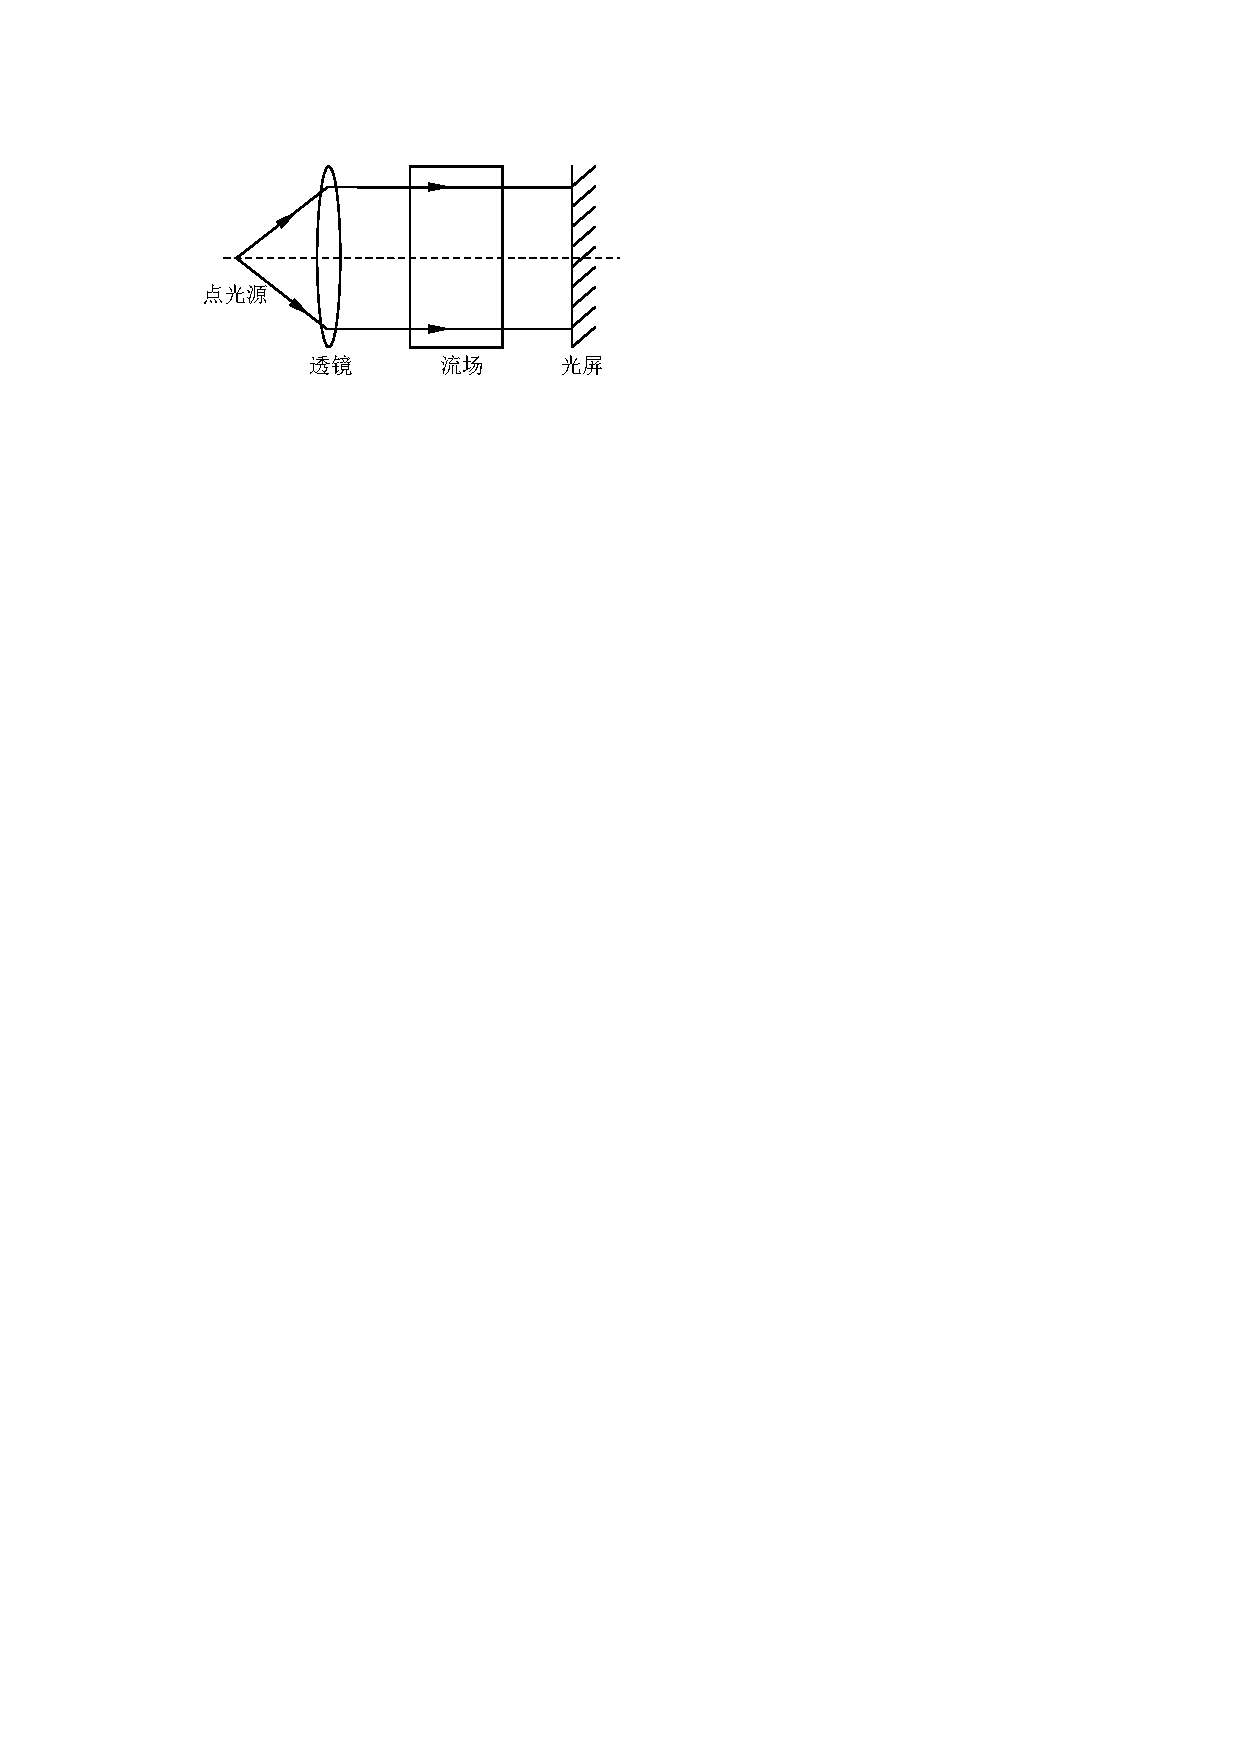
\includegraphics[width=0.9\textwidth]{shadow01.pdf}
\vspace{1em}

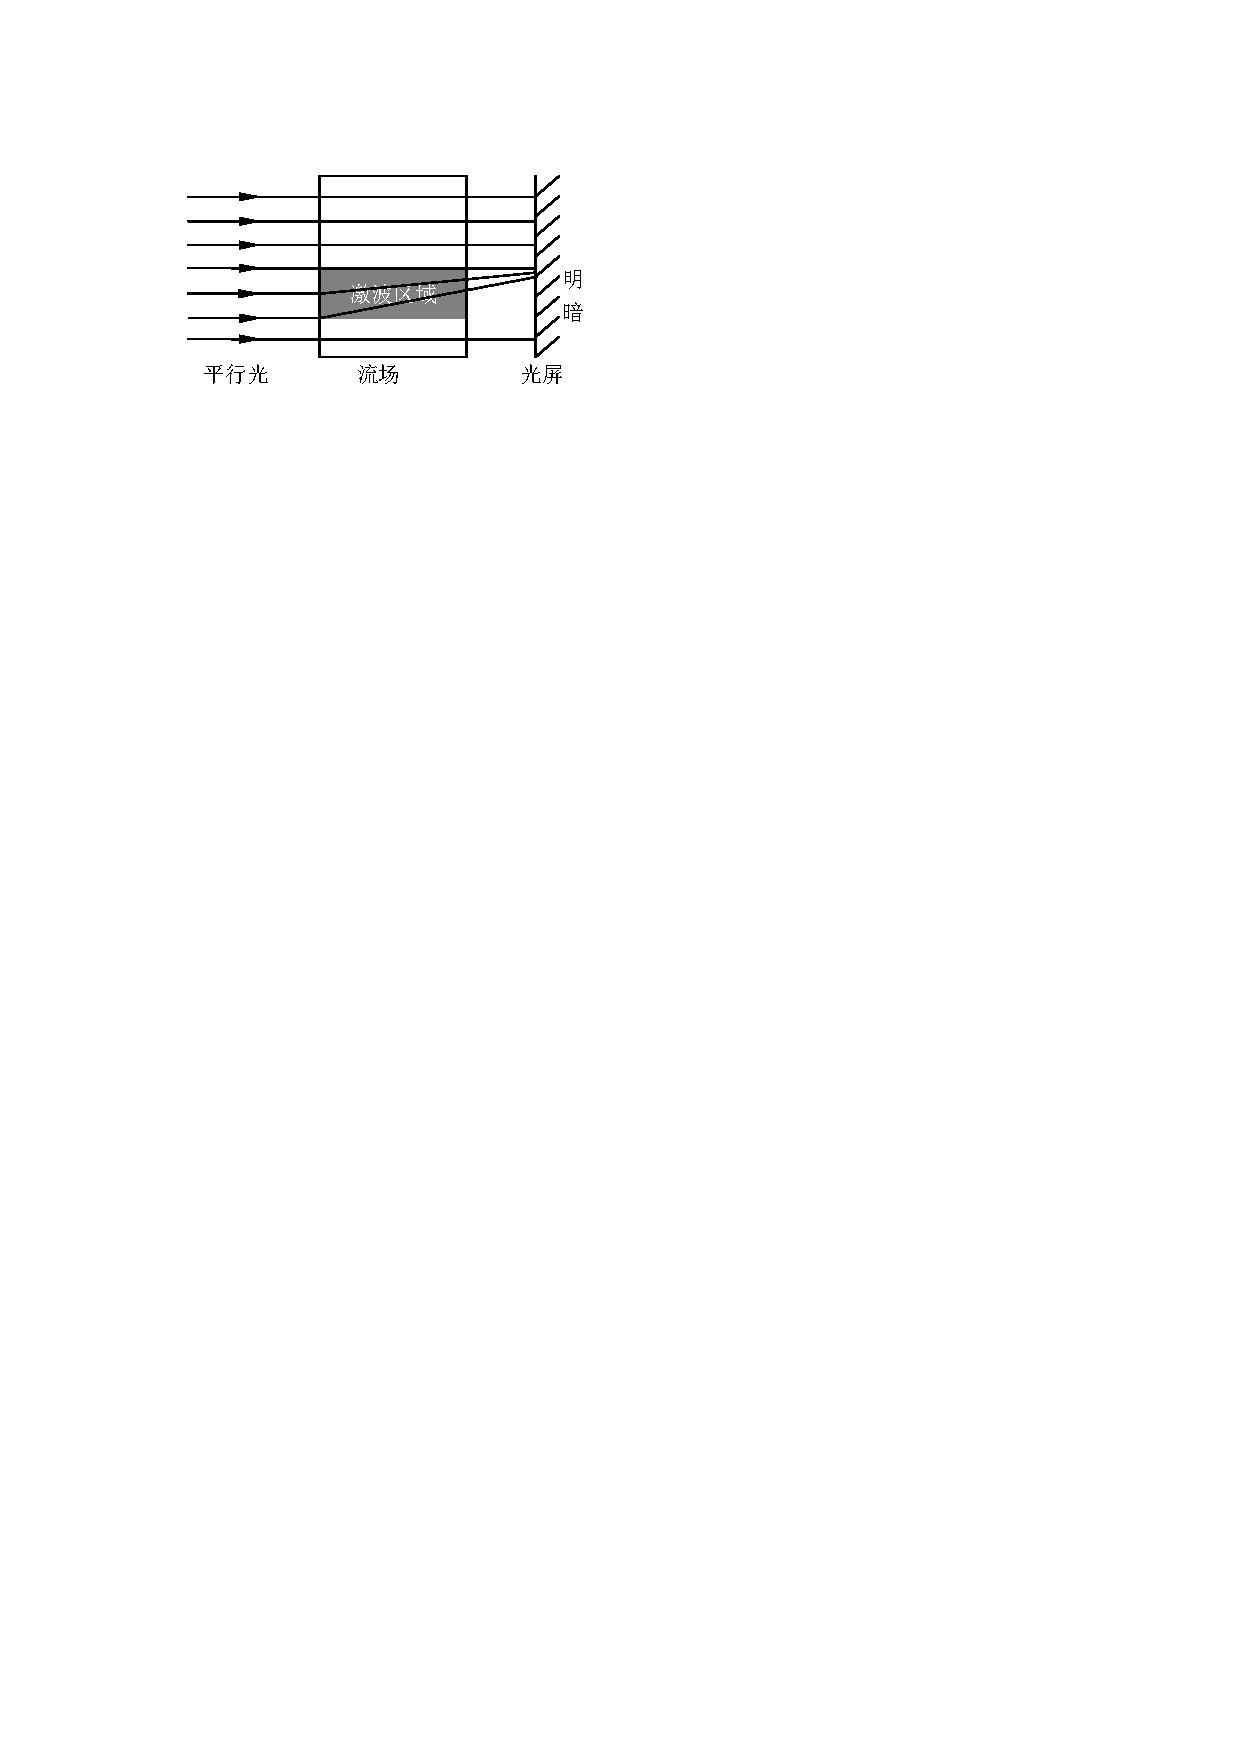
\includegraphics[width=0.91\textwidth]{shadow02.pdf}
\end{column}
\begin{column}[c]{0.5\textwidth}
\begin{itemize}
\item 流场中非激波区各点的折射率相同. 折射率的二阶导数$\partial^2n/\partial x^2=0$. 光线依然保持平行, 亮度不变.

\item 激波区存在很大的密度梯度. 在激波前锋部分,  折射率的二阶导数$\partial^2n/\partial x^2>0$, 光线散开, 屏幕上相应部分变暗.

\item 激波的后半部, 折射率的二阶导数$\partial^2n/\partial x^2<0$, 光线聚拢, 屏幕上相应部分变亮.
\end{itemize}
\end{column}
\end{columns}
}

\subsection{纹影法}
\frame{\frametitle{纹影法}
\begin{center}
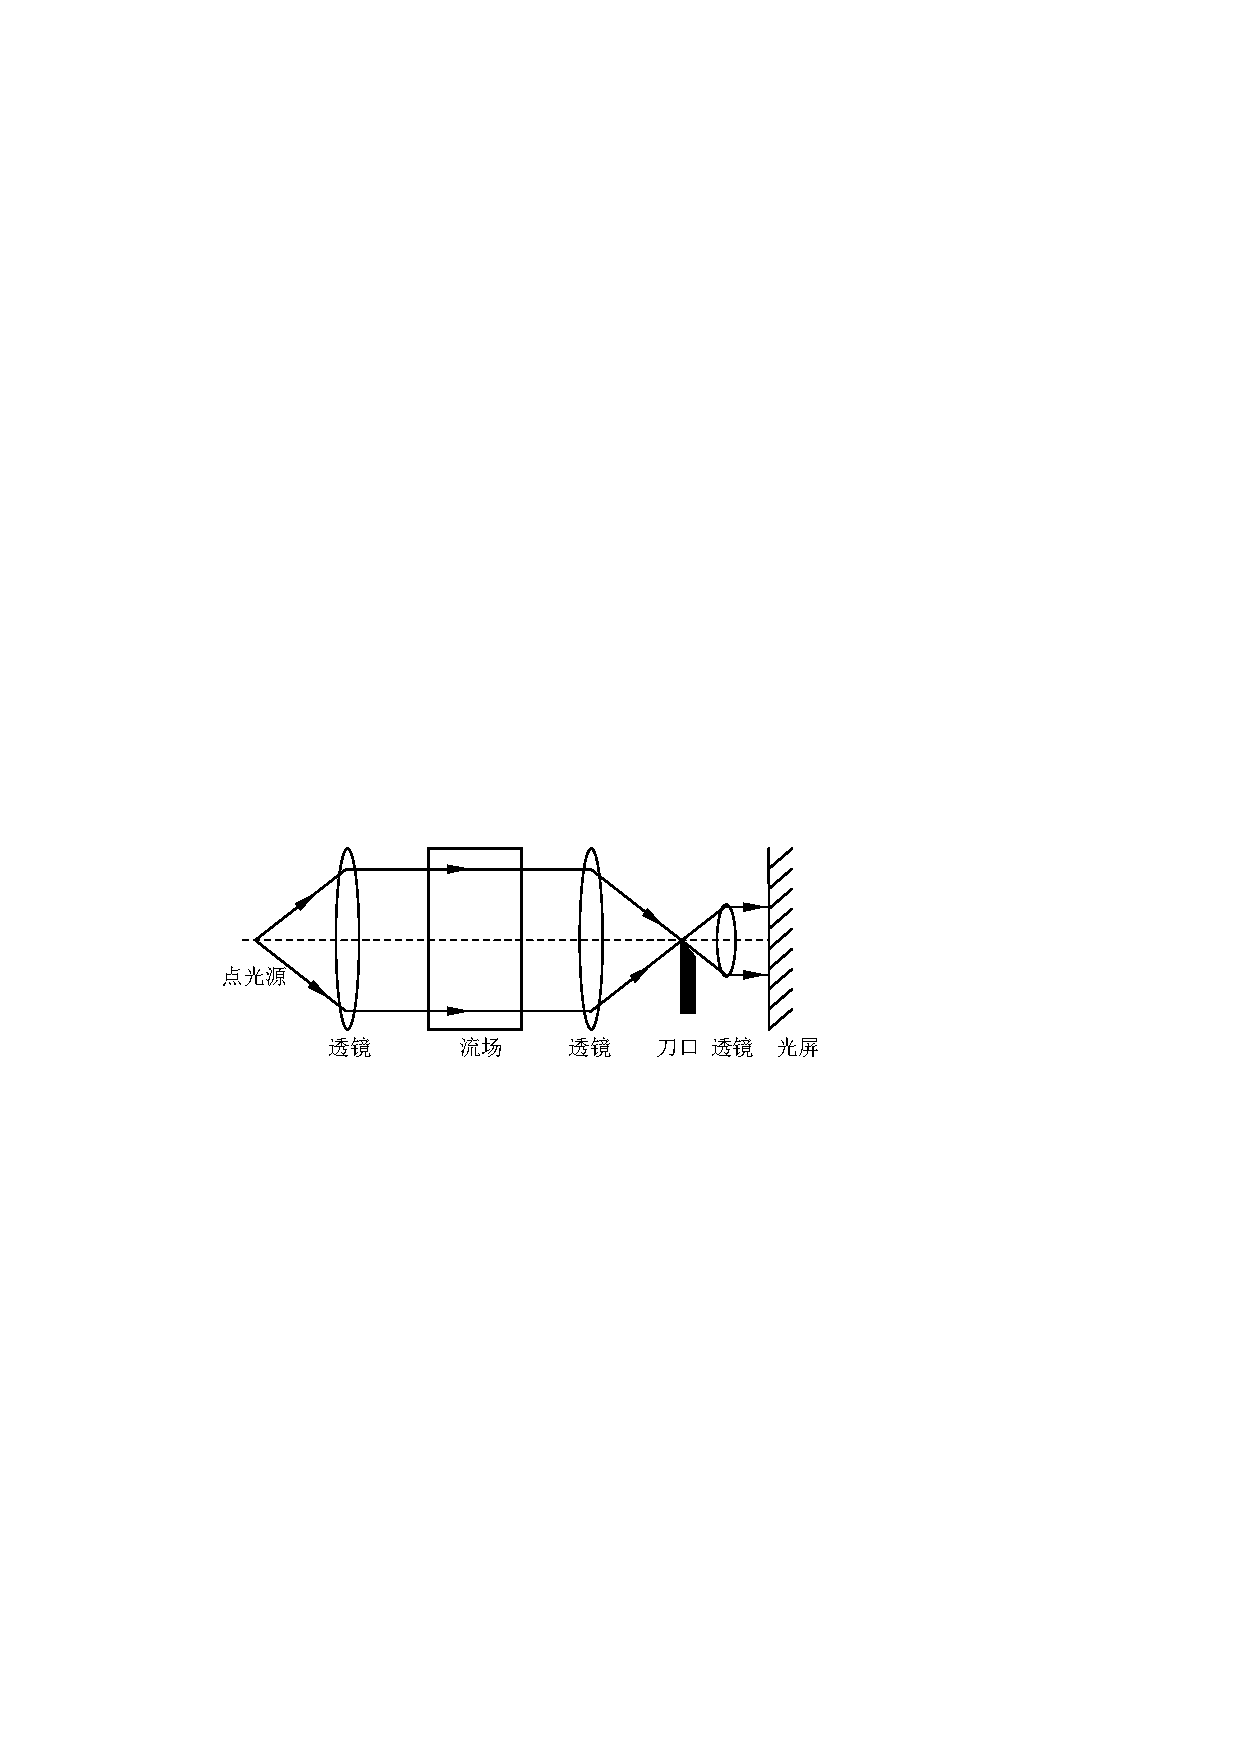
\includegraphics[width=0.8\textwidth]{schlieren01.pdf}
\end{center}

\begin{itemize}
\item 气流不均匀, 光线就会发生偏折. 向上折射$\Delta\theta$角的光线就会越过刀口光阑射到屏幕上, 幕上某些点由于额外多照射一些光线, 就比其他点亮一些.
\item 向下折射$\Delta\theta$的这部分光线就受到刀口光阑的阻挡, 幕上某些点就会比原来暗一些.
\item 屏幕上各点的阴暗程度取决于光线的偏折角$\Delta\theta$,对应于$\partial\rho/\partial x$.
\end{itemize}
}
